% Gemini theme
% https://github.com/anishathalye/gemini

\documentclass[final]{beamer}

% ====================
% Packages
% ====================

\usepackage[T1]{fontenc}
\usepackage{lmodern}
\usepackage[size=custom,width=120,height=72,scale=1.0]{beamerposter}
\usetheme{gemini}
\usecolortheme{mit}
\usepackage{graphicx}
\usepackage{booktabs}
\usepackage{bchart}
\usepackage{tikz}
\usepackage{pgfplots}
\pgfplotsset{compat=1.14}
\usepackage{anyfontsize}
\usepackage{multicol}
\usepackage{xcolor}
% ====================
% Lengths
% ====================

% If you have N columns, choose \sepwidth and \colwidth such that
% (N+1)*\sepwidth + N*\colwidth = \paperwidth
\newlength{\sepwidth}
\newlength{\colwidth}
\setlength{\sepwidth}{0.025\paperwidth}
\setlength{\colwidth}{0.3\paperwidth}

\newcommand{\separatorcolumn}{\begin{column}{\sepwidth}\end{column}}

% ====================
% Title
% ====================

\title{Estrategias para la exploración coordinada multi-VANT}

\author{Luis Alberto Ballado Aradias \and Dr. José Gabriel Ramirez-Torres \and Dr. Eduardo Arturo Rodriguez-Tello}

\institute[shortinst]{CINVESTAV - UNIDAD TAMAULIPAS}

% ====================
% Footer (optional)
% ====================

\footercontent{
  \href{https://www.tamps.cinvestav.mx/}{https://www.tamps.cinvestav.mx/} \hfill
  CINVESTAV UNIDAD TAMAULIPAS 2023 \hfill
  \href{mailto:luis.ballado@cinvestav.mx}{luis.ballado@cinvestav.mx}}
% (can be left out to remove footer)

% ====================
% Logo (optional)
% ====================

% use this to include logos on the left and/or right side of the header:
\logoright{
\includegraphics[height=7cm]{logoCinves.png}}
\logoleft{
\includegraphics[height=7cm]{cinves.png}}

% ====================
% Body
% ====================

\begin{document}

\begin{frame}[t]
\begin{columns}[t]
\separatorcolumn

\begin{column}{\colwidth}
  \begin{block}{\color{teal}\textbf{Datos VANT}}
    Leer paper https://arxiv.org/pdf/1909.01423.pdf
    \begin{multicols}{2}
    \begin{figure}[h]
      \scalebox{0.9}{
        \begin{tikzpicture}
          \begin{axis}[title  = \textbf{Valuación soluciones 2015},
              xbar,
              y axis line style = { opacity = 0 },
              axis x line       = none,
              tickwidth         = 0pt,
              ytick             = data,
              enlarge y limits  = 0.05,
              enlarge x limits  = 0.02,
              width=0.3\textwidth,
              bar width=2mm,
              symbolic y coords = {Infraestructura, Critic Count, Critic Score, User Score, Platform, Genre, Rating},
              nodes near coords,
            ]
            \addplot coordinates { (100,Infraestructura) (93,Critic Count) (57,Critic Score) (20,User Score) (10.5,Platform) (2.3,Genre) (4.52,Rating) };
          \end{axis}
        \end{tikzpicture}
      }
    \end{figure}
    
    \begin{figure}[t]
      \begin{tikzpicture}
        \begin{axis}[
	    x tick label style={
	      /pgf/number format/1000 sep=},
	    ylabel=Year,
	    enlargelimits=0.05,
	    legend style={at={(0.5,-0.1)},
	      anchor=north,legend columns=-1},
	    ybar interval=0.7,
          ]
          \addplot 
	  coordinates {(2012,408184) (2011,408348)
	    (2010,414870) (2009,412156)};
          \legend{Articulos}
        \end{axis}
      \end{tikzpicture}
    \end{figure}
    \end{multicols}
    
    \begin{multicols}{3}
      \begin{itemize}
      \item \textbf{Fusce dapibus tellus} vel tellus semper finibus. In consequat, nibh sed mattis luctus, augue diam fermentum lectus.\cite{shannon1948communication}\\
      \item \textbf{Fusce dapibus tellus} vel tellus semper finibus. In consequat, nibh sed mattis luctus, augue diam fermentum lectus.\cite{otromas}\\
      \item \textbf{Fusce dapibus tellus} vel tellus semper finibus. In consequat, nibh sed mattis luctus, augue diam fermentum lectus.\cite{unomas}\\
      \end{itemize}
    \end{multicols}
  \end{block}
  
  \begin{block}{\color{teal}Robot Autonomo}
    \heading{Another heading inside a block}
    Lorem ipsum dolor sit amet, consectetur adipiscing elit. Morbi ultricies Lorem ipsum dolor sit amet, consectetur adipiscing elit. Morbi ultricies.
    \begin{multicols}{2}
      \begin{itemize}
      \item ¿Como llego ahi?
        Some block contents, followed by a diagram, followed by a dummy paragraph.
      \item ¿Como llego ahi?
        Some block contents, followed by a diagram, followed by a dummy paragraph.
      \item ¿Como llego ahi?
        Some block contents, followed by a diagram, followed by a dummy paragraph.
      \end{itemize}
      \heading{Another heading inside a block}
      Lorem ipsum dolor sit amet, consectetur adipiscing elit. Morbi ultricies
    eget libero ac ullamcorper. Integer et euismod ante. Aenean vestibulum
    lobortis augue, ut lobortis turpis rhoncus sed. Proin feugiat nibh a
    lacinia dignissim. Proin scelerisque, risus eget tempor fermentum, ex
    turpis condimentum urna, quis malesuada sapien arcu eu purus.
      
    \begin{figure}
      \centering
      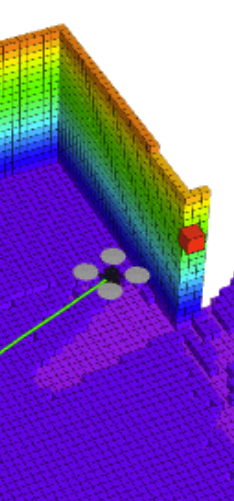
\includegraphics[width=10cm]{images/drone_vuelo.png}
      \end{figure}
    \end{multicols}
    Lorem ipsum dolor sit amet, consectetur adipiscing elit. Morbi ultricies
    eget libero ac ullamcorper. Integer et euismod ante. Aenean vestibulum
    lobortis augue, ut lobortis turpis rhoncus sed. Proin feugiat nibh a
    lacinia dignissim. Proin scelerisque, risus eget tempor fermentum, ex
    turpis condimentum urna, quis malesuada sapien arcu eu purus.

  \end{block}
\end{column}

\separatorcolumn

\begin{column}{\colwidth}
  
  \begin{block}{\color{teal}Taxonomia VANT Multi-rotor}
        
    \begin{enumerate}
      \item \textbf{Algo aqui}, egestas at vehicula et, convallis
        accumsan orci. Orci varius natoque penatibus et magnis dis parturient
        montes, nascetur ridiculus mus.
      \item \textbf{Cras vehicula blandit urna ut maximus}. Aliquam blandit nec
        massa ac sollicitudin. Curabitur cursus, metus nec imperdiet bibendum,
        velit lectus faucibus dolor, quis gravida metus mauris gravida turpis.
      \item \textbf{Vestibulum et massa diam}. Phasellus fermentum augue non
        nulla accumsan, non rhoncus lectus condimentum.
    \end{enumerate}

    \begin{figure}[t]
      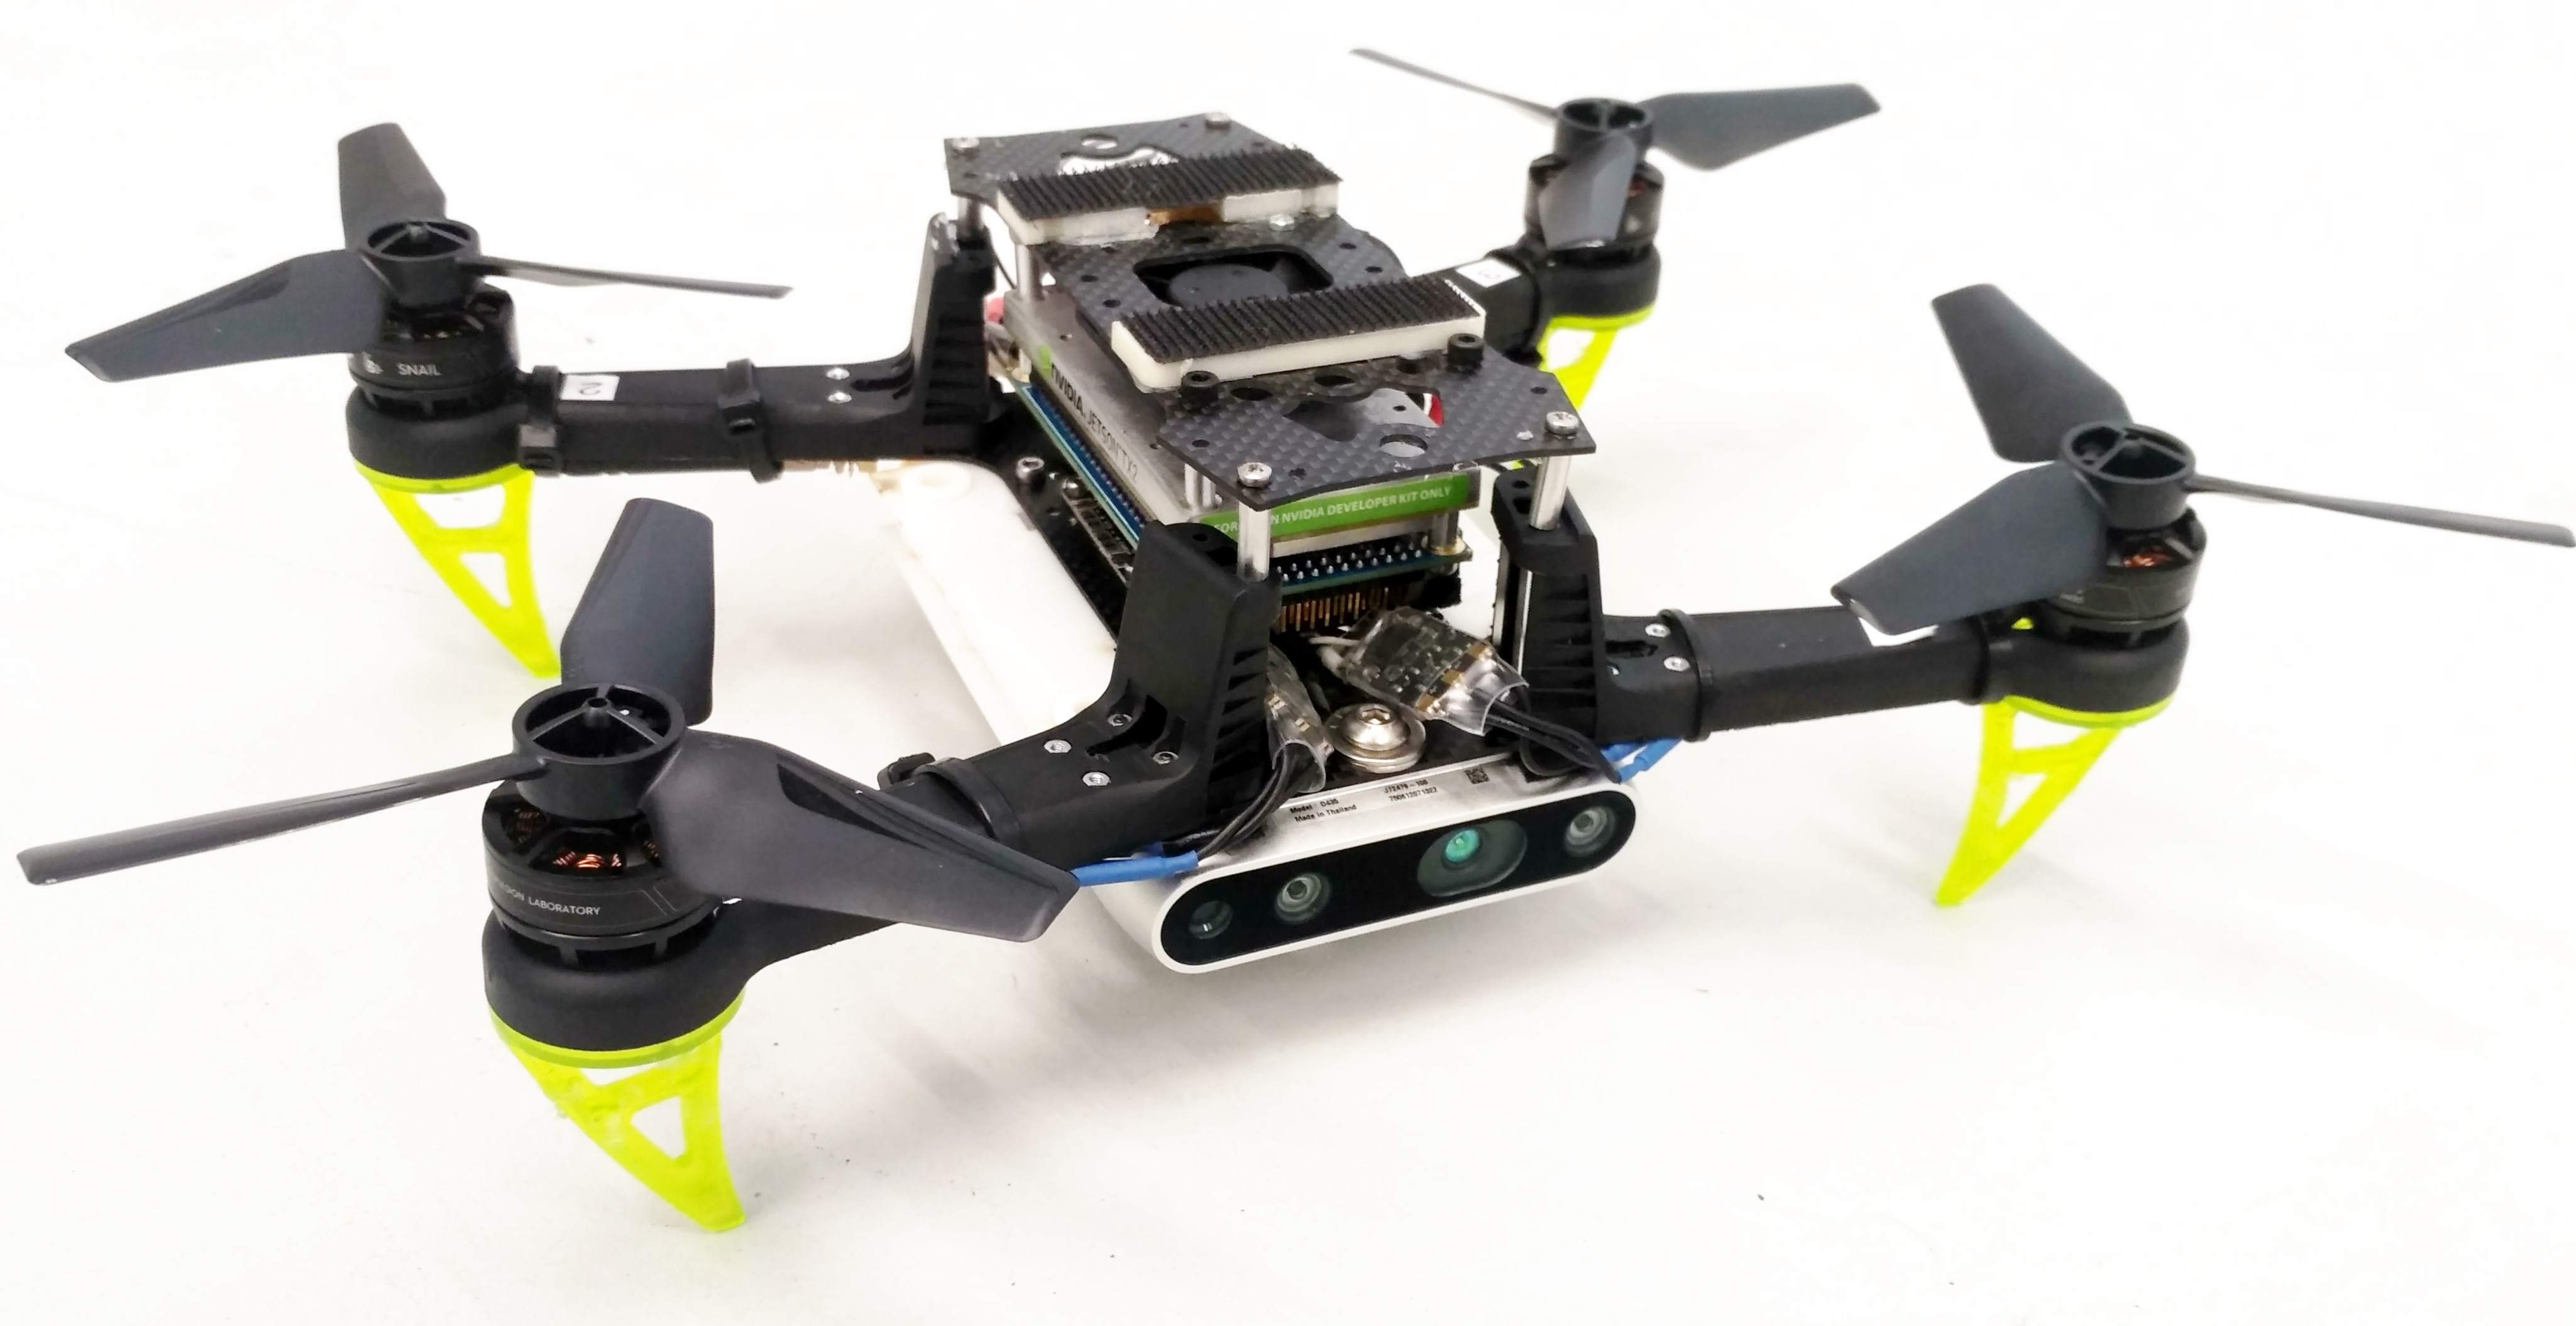
\includegraphics[width=38cm]{images/uav_planning_drone.jpg}
      \centering
    \end{figure}
    
  \end{block}
  
  \begin{block}{\color{teal}Arquitectura Busqueda y Rescate}
    
    Nulla eget sem quam. Ut aliquam volutpat nisi vestibulum convallis. Nunc a
    lectus et eros facilisis hendrerit eu non urna. Interdum et malesuada fames
    ac ante \textit{ipsum primis} in faucibus. Etiam sit amet velit eget sem
    euismod tristique. Praesent enim erat, porta vel mattis sed, pharetra sed
    ipsum. Morbi commodo condimentum massa, \textit{tempus venenatis} massa
    hendrerit quis. Maecenas sed porta est. Praesent mollis interdum lectus,
    sit amet sollicitudin risus tincidunt non.

    \begin{itemize}
    \item \textbf{Sed consequat} id ante vel efficitur. Praesent congue massa
      sed est scelerisque, elementum mollis augue iaculis.
      \begin{itemize}
      \item In sed est finibus, vulputate
        nunc gravida, pulvinar lorem. In maximus nunc dolor, sed auctor eros
        porttitor quis.
      \item Fusce ornare dignissim nisi. Nam sit amet risus vel lacus
        tempor tincidunt eu a arcu.
      \item Donec rhoncus vestibulum erat, quis aliquam leo
        gravida egestas.
      \end{itemize}
    \item \textbf{Sed luctus, elit sit amet} dictum maximus, diam dolor
      faucibus purus, sed lobortis justo erat id turpis.
    \item \textbf{Pellentesque facilisis dolor in leo} bibendum congue.
      Maecenas congue finibus justo, vitae eleifend urna facilisis at.
    \end{itemize}
    
  \end{block}

\end{column}

\separatorcolumn

\begin{column}{\colwidth}
  
  \begin{block}{\color{teal}Aplicaciones}

    \begin{figure}
      \centering
      
\includegraphics[width=30cm]{images/drone_usos.png}
      \end{figure}
    
    
  \end{block}

  \begin{block}{\color{teal}Estrategia exploración coordinada}

    \begin{figure}
      \centering
      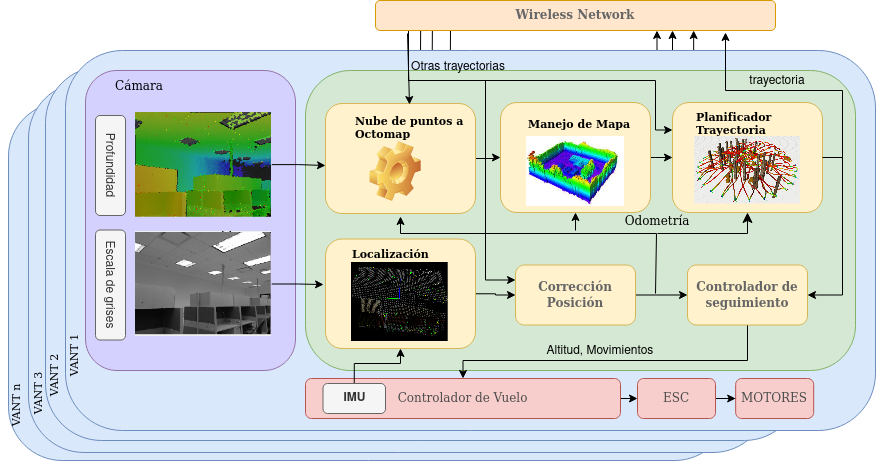
\includegraphics[width=35cm]{images/arquitectura.png}
    \end{figure}

    \begin{figure}
      \centering
      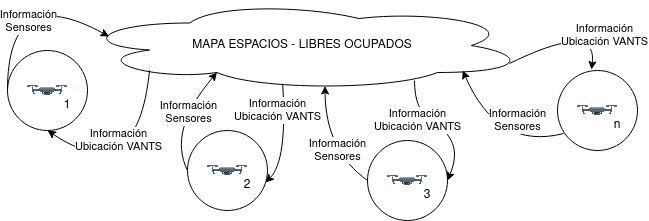
\includegraphics[width=35cm]{images/problema.png}
      \end{figure}
    

  \end{block}

  \begin{block}{\color{teal}Referencias}

    \nocite{*}
    \footnotesize{\bibliographystyle{plain}\bibliography{poster}}

  \end{block}

\end{column}

\separatorcolumn
\end{columns}
\end{frame}

\end{document}
